\documentclass[ukenglish]{nik}
\usepackage{mathptm}
\usepackage{hyperref}
\usepackage{amsfonts,amsmath,amssymb,amstext}
\usepackage{latexsym}
\usepackage{graphicx}
\usepackage{url,alltt}

\newcommand{\va}{\mathit{variable}}
\newcommand{\Fa}{\mathrm{F}}
\newcommand{\TEXT}{{\mathrm{TEXT}}}
\newcommand{\Nat}{\mathbb{N}}
\newcommand{\Int}{\mathbb{Z}}
\newcommand{\Rat}{\mathbb{Q}}
\newcommand{\Rea}{\mathbb{R}}
\newcommand{\cS}{\mathcal{S}}
\newcommand{\cD}{\mathcal{D}}
\newcommand{\cT}{\mathcal{T}}
\newcommand{\cL}{\mathcal{L}}
\newcommand{\cB}{\mathcal{B}}
\newcommand{\cF}{\mathcal{F}}
\newcommand{\cN}{\mathcal{N}}
\newcommand{\cP}{\mathcal{P}}
\newcommand{\cA}{\mathcal{A}}
\newcommand{\ra}{\rightarrow}
\newcommand{\Ra}{\Rightarrow}
\newcommand{\set}[1]{\{#1\}}
\newcommand{\seg}[2]{[#1.\,.#2]}
\newcommand{\pair}[2]{\langle #1,#2\rangle}
\newcommand{\der}[2]{\frac{\partial#1}{\partial#2}}
\newcommand{\plusD}[1]{#1+\Delta{#1}}
\newcommand{\dD}[1]{\Delta{#1}}
\newcommand{\range}{\mathit{range}}
\newcommand{\oa}{\overline{a}}
\newcommand{\ob}{\overline{b}}
\newcommand{\oc}{\overline{c}}
\newcommand{\oz}{\overline{\zeta}}
\newcommand{\ea}{\epsilon_1}
\newcommand{\eb}{\epsilon_2}
\newcommand{\ec}{\epsilon_3}
\newcommand{\ba}{\frac{100}{2}b_1}
\newcommand{\bb}{\frac{10}{2}b_2}
\newcommand{\bc}{\frac{1}{2}b_3}
\newcommand{\binomsq}[2]{\left[\begin{array}{c}#1\\#2\end{array}\right]}



\begin{document}

\title{\url{pplex} - A Tool for Teaching the Simplex Method}

\author{
Joanna Bauer\thanks{University of Bergen, Department of Informatics, P.O.Box 7803, N-5020 Bergen, Norway}
\and
Marc Bezem$^*$
\and
Andreas Halle$^*$}

\maketitle

\begin{abstract}
Linear programs occur frequently in various important disciplines, such as economics, management, and engineering.
The simplex method is the best known and most widely used method to solve linear programs.
Therefore, it is taught to a wide range of students with varying background in mathematics.
We present the software \url{pplex} for supporting
the classroom presentation of the simplex method.
Distinctive features of our tool are: 
portability, 
simple command line interface, 
file input in standard LP format,
geometric interpretation (two variables).
\end{abstract}

\section{Introduction and Motivation}\label{sec:intro}
In an optimization problem, the objective is to decide on how to utilize given resources such that they maximize some ``profit'' (or minimize some ``cost''), while satisfying a set of additional constraints on the resources.
This is commonly modelled by associating the possible decisions with variables, such that the profit and the constraints can be formulated as functions of these variables. 
If the profit function, the so-called \emph{objective (function)}, is linear and the constraints can be formulated as linear (in)equalities, then the optimization problem has a \emph{linear programming (LP)} formulation. A specific instance of an LP formulation is called a \emph{linear program}.
A linear program is solved by identifying those values for the variables that maximize the objective while satisfying all constraints.
Linear programs occur frequently in economics, management, and engineering.

The simplex method is by far the most widely used method for solving linear programs. 
It is listed as one of the top 10 algorithms of the twentieth century in
\cite{CiSaE2000}. Given the many applications of LP, the simplex method is taught to a wide range of
students, including students with a weak background in mathematics and algorithms. 

Most lecturers on linear programming need to demonstrate the simplex method step-by-step 
\emph{without being distracted by detailed calculations in elementary linear algebra}. Let us start by
introducing the simplex method by a simple example:
\[
    \begin{array}{lrcrcrl}
			\text{Maximize}  &    x &+&    y &	&	& \quad\quad \text{(objective function)}\\
			\text{subject to}&  2 x &+&    y &\leq&   6	& \quad\quad \text{(constraint)}\\
    	\text{and}&         7 x &+& 13 y &\leq&  40 & \quad\quad \text{(constraint)}\\
    	\text{and}       &    x &,&    y &\geq&0    &\quad\quad \text{(two constraints)}
    \end{array}
\]
where the variables $x$ and $y$ range over the real numbers.

A \emph{feasible} point is an assignment of real numbers to the variables 
such that all constraints are satisfied. 
The inequality constraints correspond to halfspaces (here halfplanes), and the constraints of a program 
define the \emph{polyhedron} containing the feasible points.
In the example above there exist feasible points,
since the polyhedron given by the four inequalities contains,
among other points, the origin  (see Figure~\ref{fig:ex1}). 

\begin{figure}[htb]
	\begin{center}
		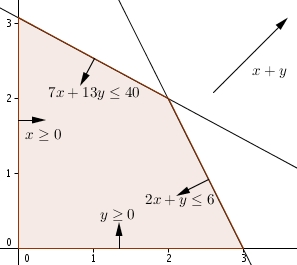
\includegraphics{ex1.jpg}
	\end{center}
	\caption{Geometric interpretation of our example linear program}
	\label{fig:ex1}
\end{figure}

Since inequalities cannot be manipulated algebraically as easily
as equations, a first step is to reformulate the program such that it is expressed
by linear equations in combination with simple inequalities of the form
$\mathit{variable}\geq 0$. For this purpose, we introduce
two new variables, here $u$ and $v$, called \emph{slack variables}, 
measuring to what extent the linear inequalities are satisfied. 
We also introduce a new variable $\zeta$
for the objective function $x+y$. 
Thus our linear program is brought into the following form, 
called a \emph{dictionary} in \cite{Vanderbei}:
\[    
    \begin{array}{lcrcrcrcr}
      \zeta&=&   & &     x &+&     y & &  \\\hline
      u    &=& 6 &-&   2 x &-&     y & &  \\
      v    &=& 40&-&   7 x &-&  13 y & &  \\
      x,y,u,v  &\geq&0     & &  & &  & &    
    \end{array}
\]

Since we now deal with two equalities in four variables, 
assigning values to any variable pair determines the values of the remaining two variables.

Geometric considerations lead to the observation that the
maximal value of the objective subject to the constraints (linear
equalities and inequalities of the form 
$\mathit{variable}\geq 0$) is attained in a vertex of the polyhedron. 
Through the introduction of the slack variables, each edge of the polyhedron now corresponds to one variable
being zero. Thus assigning zero to a pair of variables corresponds to the intersection point of the corresponding pair of edges. 
This intersection point either lies outside the polyhedron (f.ex. for $y=v=0$), or  
it is a vertex of the polyhedron and thus a potential candidate for the optimal solution. 
For this reason, we are especially interested in assignments to $(x,y,u,v)$ where two variables are set to zero. 
Such an assignment is called a \emph{basic solution}. The variables being zero are called \emph{non-basic} variables.

Every basic solution corresponds to a dictionary with the non-basic variables on the right side of ``='', 
enforcing the variables on the left (the \emph{basic} variables) to equal the constants in the equations. 
If one of the constants is negative, then the corresponding basic solution is not feasible. 
(Geometrically, a non-feasible basic solution lies outside of the polyhedron with respect to 
the inequality corresponding to the variable that is assigned a negative value.)
We  call a dictionary \emph{(in)feasible} if the corresponding basic solution is (not) feasible.

In the example above, we start in the origin $x=y=0$ and get
value $0$ for the objective $\zeta = x + y$.
Clearly, there is room for improvement here, since in fact
the value $0$ is the \emph{minimal} value of the objective
under the given constraints. How can we improve on this
value? The answer is simple: increase $x$ or $y$ or both.
The simplex method chooses one non-basic variable and
tries to increase it as much as possible, while keeping the
other non-basic variables constant zero.
Let's try to increase $x$ keeping $y=0$. How much can $x$ increase?
We see that $0 \leq u = 6 -2x-y$ allows us to increase $x$ to $3$,
and that the other linear equation allows an even larger increase. Since both
$u\geq 0$ and $v\geq 0$ must be respected, we increase $x$ to $3$,
thereby getting $u=0$ as a consequence. Moreover, the objective $x+y$ evaluates to 3.

With its value increased to $3$, variable $x$ doesn't qualify as a non-basic variable anymore.
Fortunately, the variable $u$ has become zero. Interchanging the roles of
$x$ and $u$ as non-basic and basic variable, respectively, restores 
the invariant of the dictionary form. The limiting equation $u = 6 -2x-y$ makes it
possible to express $x$ in $u$ and $y$ such that $x$ can be eliminated from the
right-hand side of the dictionary form. The equation $u = 6 -2x-y$ is
called the \emph{pivot} and interchanging the roles of
a basic and a non-basic variable is called \emph{pivoting}.
In the dictionary, pivoting is done by standard row operations in linear algebra. 
The incumbent dictionary becomes:

	\begin{minipage}{.45\textwidth}
\[    
    \begin{array}{lcrcrcrcr}
      \zeta&=& 3 &-& 0.5 u &+& 0.5 y & &  \\\hline
      x    &=& 3 &-& 0.5 u &-& 0.5 y & &  \\
      v    &=& 19&+& 3.5 u &-& 9.5 y & &  \\

    \end{array}
\]
\end{minipage}
	\begin{minipage}{.45\textwidth}
				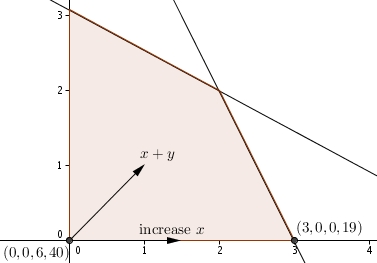
\includegraphics{ex2.jpg}
\end{minipage}
\vspace{.2cm}

The next step
starts by observing that the objective improves if we 
increase $y$ while keeping $u$ constant zero. We see that
$0\leq v = 19 + 3.5u - 9.5y$ allows to increase $y$ to $2$,
and that the other equation allows an even larger increase.
Hence, we pivot $y$ and $v$ using the second equation.
The incumbent dictionary becomes:
\vspace{.2cm}
	\begin{minipage}{.45\textwidth}
\[    
    \begin{array}{lcrcrcrcr}
      \zeta&=& 4 &-& \frac{6}{19} u &-& \frac{1}{19} v &\vphantom{\frac{|}{|}} &  \\\hline
      x    &=& 2 &-&\frac{13}{19} u &+& \frac{1}{19} v &\vphantom{\frac{|}{|}} &  \\
      y    &=& 2 &+& \frac{7}{19} u &-& \frac{1}{19} v &\vphantom{\frac{|}{|}} &  \\
    \end{array}
\]
\end{minipage}
	\begin{minipage}{.45\textwidth}
				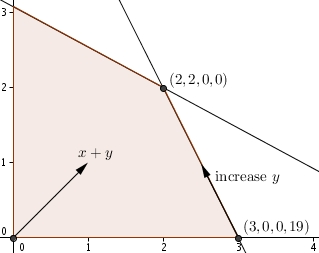
\includegraphics{ex3.jpg}
\end{minipage}
\vspace{.2cm}

The good news is that we have found the maximum, as all coefficients in the objective
are negative. The maximum value $4$
of the objective is attained in the point $x=y=2$. These values are 
integers by the design of the example, and can also be obtained graphically.
Obtaining the last dictionary algebraically is a painful (but useful) exercise.

An interested student may now ask the question: 
Can't we start with $y$ instead of with $x$?
This very good question deserves a detailed answer.
The lecturer (our hero) starts boldly calculating on the blackboard.
Clearly, $0\leq v = 40 - 7x -13y$ allows us to increase $y$ to $\frac{40}{13}$,
and the other linear equation allows an even larger increase. Hence we pivot and get,
again by standard row operations, the new dictionary:
\begin{minipage}{.63\textwidth}
\[    
    \begin{array}{lcrcrcrcr}
      \zeta&=& \frac{40}{13} &+& \frac{6}{13} x &-& \frac{1}{13} v &\vphantom{\frac{|}{|}} &  \\\hline
      u    &=& \frac{38}{13} &-&\frac{19}{13} x &+& \frac{1}{13} v &\vphantom{\frac{|}{|}} &  \\
      y    &=& \frac{40}{13} &-& \frac{7}{13} x &-& \frac{1}{13} v &\vphantom{\frac{|}{|}} &  \\
    \end{array}
\]
At this point the lecturer almost regrets his willingness to answer the student's
question in detail, but manages as by miracle to finally produce the following dictionary:
\[    
    \begin{array}{lcrcrcrcr}
      \zeta&=& 4 &-& \frac{6}{19} u &-& \frac{1}{19} v &\vphantom{\frac{|}{|}} &  \\\hline
      x    &=& 2 &-&\frac{13}{19} u &+& \frac{1}{19} v &\vphantom{\frac{|}{|}} &  \\
      y    &=& 2 &+& \frac{7}{19} u &-& \frac{2}{19} v &\vphantom{\frac{|}{|}} &  \\
    \end{array}
\]
\end{minipage}
	\begin{minipage}{.32\textwidth}
				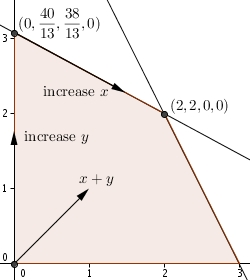
\includegraphics{ex4.jpg}
\end{minipage}
\vspace{.2cm}

A Happy End? Not yet. Some attentive students point out that the two final dictionaries
are not completely identical and ask for an explanation. After some discussion, it turns
out that the fraction $\frac{2}{19}$ in the (last) final dictionary is correct,
and that the corresponding fraction $\frac{1}{19}$ in the (previous) final dictionary was wrong.
The mistake may have gone unnoticed, since it didn't spoil the answer, the maximum stays
$4$ at $x=y=2$. However, the mistake may have confused a student working through the details at a later moment.

What do we conclude from the above example? It is certainly useful to demonstrate some
linear algebra calculations explicitly. Nevertheless, linear algebra should be a prerequisite for a course
in linear programming. The details of linear algebra should not distract from the important
issues in linear programming. These issues include:
\begin{itemize}
\item The choice of the pivot.
\item What if the initial dictionary is not feasible?
\item Duality theory.
\item Efficiency considerations.
\item Sensitivity analysis.
\item Important special cases such as network problems.
\end{itemize}
Even for simple examples it is unnatural (and often impossible)
to design them in such a way that the linear algebra calculations stay simple.
A computerized tool for these calculations facilitates their demonstration.
The benefits of such a tool are three-fold: no precious class-room time is wasted
on elementary calculations, no calculation errors distract attention, and
the demonstration of larger, more interesting examples becomes feasible.
There is also a danger associated with the use of such tools in teaching: 
one should make sure that the students really understand the elementary
calculations the tool is performing. The idea of having a tool
for experimenting with the simplex method is, of course, not new. 
See, for example, \cite{SimplexPivotTool, AdvancedPivotTool}.
However, tools tend to gradually go out-of-date on newer platforms
than those used to develop them. Distinctive features of our tool are: 
portability, 
simple command line interface, 
file input in standard LP format,
geometric interpretation (two variables, so far).

This paper is organized as follows.
In Section~\ref{sec:pplex} we introduce 
our tool \url{pplex}, applied to several examples in Section~\ref{sec:examples}.
We conclude by discussing ongoing work in Section~\ref{sec:future}.

\section{A tool for teaching the Simplex method}\label{sec:pplex}
Our contribution \url{pplex}~\cite{pplex},
a \emph{pedagogical implementation of the Simplex method},
is free software distributed under the GNU General Public License \cite{GNUGPL}.
It runs under Java 6 and Java 7 and is portable to any supportive platform.

We start by demonstrating \url{pplex} on the example from the introduction.
The input file for our example reads:
\begin{alltt}
\documentclass[10pt]{article}
\usepackage[utf8]{inputenc}
\usepackage{pgf,tikz}
\usetikzlibrary{arrows}
\pagestyle{empty}
\begin{document}
\begin{tikzpicture}[line cap=round,line join=round,>=triangle 45,x=1.0cm,y=1.0cm]
\draw[->,color=black] (-4.3,0) -- (7.52,0);
\foreach \x in {-4,-2,2,4,6}
\draw[shift={(\x,0)},color=black] (0pt,2pt) -- (0pt,-2pt) node[below] {\footnotesize $\x$};
\draw[->,color=black] (0,-3.14) -- (0,6.3);
\foreach \y in {-2,2,4,6}
\draw[shift={(0,\y)},color=black] (2pt,0pt) -- (-2pt,0pt) node[left] {\footnotesize $\y$};
\draw[color=black] (0pt,-10pt) node[right] {\footnotesize $0$};
\clip(-4.3,-3.14) rectangle (7.52,6.3);
\draw [domain=-4.3:7.52] plot(\x,{(--4.5-1*\x)/1});
\draw [domain=-4.3:7.52] plot(\x,{(--40-7*\x)/13});
\draw [domain=-4.3:7.52] plot(\x,{(--6-2*\x)/1});
%\draw (0,-3.14) -- (0,6.3); MB outcomment
%\draw [domain=-4.3:7.52] plot(\x,{(-0-0*\x)/1}); MB outcomment
%Marc starts having fun
{\foreach \x in {0,0.2,...,6} 
  {\foreach \y in {0,0.2,...,6}
    {\pgfmathparse{2*\x+\y < 6 && 7*\x + 13*\y < 40}
      \ifnum\pgfmathresult=1{\draw[color=red](\x,\y) node {$\cdot$};}\fi}}}

\end{tikzpicture}
\end{document}
\end{alltt}
Note that the inequalities $x,y \geq 0$ are implicitly assumed, and omitted in both the input file and the generated dictionaries.

The program \url{pplex} launches with the prompt \verb|pplex>|.
We read the above input file, which is confirmed OK:
\begin{verbatim}
pplex> read input/nik2.lps
Read input/nik2.lps OK.
\end{verbatim}
To show the initial dictionary of this program one writes after the prompt:
\begin{alltt}
pplex> show
 \(\zeta\) =       +     x +      y
w1 =  6.00 - 2.00x -      y
w2 = 40.00 - 7.00x - 13.00y
\end{alltt}
Numbers are by default displayed with two decimals precision, whereas
calculations are performed in double precision arithmetic.
We can now let \url{pplex} execute a pivot by specifying
the variable by its \emph{column} (here $1$ for $x$ and $2$ for $y$)
and the linear equation by its \emph{row}. 
Here comes the command and the resulting dictionary:
\begin{alltt}
pplex> pivot 1 1
 \(\zeta\) =  3.00 - 0.50w1 + 0.50y
 x =  3.00 - 0.50w1 - 0.50y
w2 = 19.00 + 3.50w1 - 9.50y
\end{alltt}
The final (optimal) dictionary is calculated after the next command:
\begin{alltt}
pplex> pivot 2 2
 \(\zeta\) = 4.00 - 0.32w1 - 0.05w2
 x = 2.00 - 0.68w1 + 0.05w2
 y = 2.00 + 0.37w1 - 0.11w2
\end{alltt}
Responding to the question of the student about starting with variable $y$, 
one can roll back to the first dictionary by two \verb|undo|'s and pivot
with $y$ and the second linear equation:
\begin{alltt}
pplex> undo

pplex> undo

pplex> pivot 2 2
 \(\zeta\) = 3.08 + 0.46x - 0.08w2
w1 = 2.92 - 1.46x + 0.08w2
 y = 3.08 - 0.54x - 0.08w2
\end{alltt}
In an effortless way one now obtains the same final dictionary:
\begin{alltt}
pplex> pivot 1 1 
 \(\zeta\) = 4.00 - 0.32w1 - 0.05w2
 x = 2.00 - 0.68w1 + 0.05w2
 y = 2.00 + 0.37w1 - 0.11w2
\end{alltt}
Due to (or despite?) the double precision arithmetic, one obtains exactly the same result.

\section{Examples of Using \texttt{pplex}}\label{sec:examples}
In this section we present examples using duality and examples illustrating
degeneracy, cycling and unboundedness.

\subsection{Duality}

Giving an introduction into LP duality theory is beyond the scope of this work. We therefore assume knowledge of duality theory throughout this section.

In Sections \ref{sec:intro} and \ref{sec:pplex}, we studied an example of an initially feasible dictionary.
What if the initial dictionary is not feasible, that is, if the origin is not a
feasible solution? Here is an example:

\begin{minipage}{.45\textwidth}
\begin{alltt}
\input{../input/nik8.lps}
\end{alltt}
\end{minipage}
\begin{minipage}{.45\textwidth}
	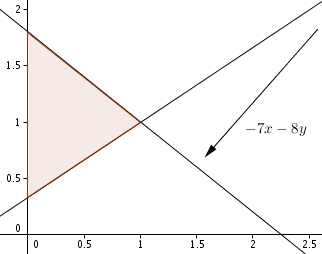
\includegraphics{ex_dual.jpg}
\end{minipage}
\vspace{.2cm}

The feasible region of this program is the
triangle with points $(0,\frac{1}{3}),(0,1.8),(1,1)$
in the $x,y$-plane, on which we maximize the objective $-7x-8y$.
Clearly, the solution $-\frac{8}{3}$ is to be found in the point $(0,\frac{1}{3})$.
However, we cannot proceed as in the previous section since the
initial dictionary is not feasible:
\begin{alltt}
pplex> read input/nik8.lps
Read input/nik8.lps OK.

pplex> show primal
 \(\zeta\) =        - 7.00x - 8.00y
w1 = - 1.00 - 2.00x + 3.00y
w2 =   9.00 - 4.00x - 5.00y
\end{alltt}
One possible approach in such a case is to solve the dual instead:
\begin{alltt}
pplex> show dual
-\(\xi\) =      +     y1 - 9.00y2
z1 = 7.00 + 2.00y1 + 4.00y2
z2 = 8.00 - 3.00y1 + 5.00y2
\end{alltt}
The negative coefficients of the original objective $-7x-8y$ show up in the dual
dictionary as the positive constants $7.00$ and $8.00$ of the first and the second 
linear equation, respectively. Since they are positive, the dual dictionary is feasible.
The maximum value $\frac{8}{3}$ of \(-\xi\) in the dual program is found after one pivot:
\begin{alltt}
pplex> pivot dual 1 2
-\(\xi\) =  2.67 - 0.33z2 - 7.33y2
z1 = 12.33 - 0.67z2 + 7.33y2
y1 =  2.67 - 0.33z2 + 1.67y2
\end{alltt}
The primal version of this dictionary shows that we have indeed found the
maximum $-\frac{8}{3}$ of $\zeta$ for $x=0,~y=\frac{1}{3}$ in the primal program:
\begin{alltt}
pplex> show primal
 \(\zeta\) = - 2.67 - 12.33x - 2.67w1
 y =   0.33 +  0.67x + 0.33w1
w2 =   7.33 -  7.33x - 1.67w1
\end{alltt}

In the last example, the dual dictionary was feasible. If both the primal and
the dual dictionary are infeasible, the linear program is solved in two phases: In the first phase,
we modify the linear program into one which \emph{is} dually feasible, by substituting all coefficients in the objective with negative values.
By solving the modified dual program we find a feasible solution of the original primal
program. In the second phase, we solve the original primal program starting from the 
feasible solution found in the first phase.
The two phases are demonstrated in \url{pplex} by the following example:
\begin{alltt}
pplex> show primal
 \(\zeta\) =        + 2.00x + y
w1 = - 1.00 -     x + y
w2 =   2.00 -     x - y
\end{alltt}
The objective is negated by \verb|replace -2 -1|,
yielding the dually feasible dictionary:
\begin{alltt}
pplex> replace -2 -1
 \(\zeta\)  =        - 2.00x - y
w1 = - 1.00 -     x + y
w2 =   2.00 -     x - y
\end{alltt}
The commands \verb|pivot dual 1 2| and \verb|show primal|
yield the feasible final dictionary:
\begin{alltt}
 \(\zeta\) = - 1.00 - 3.00x - w1
 y =   1.00 +     x + w1
w2 =   1.00 - 2.00x - w1
\end{alltt}
This is now a mock solution since the original objective was $2x+y$,
not $-2x-y$. Now the original objective must be reinstated,
replacing basic variables by their right-hand sides: $2x+y = 2x+(1+x+w_1)$.
This is achieved by the command \verb|reinstate|:
\begin{alltt}
pplex> reinstate
 \(\zeta\) = 1.00 + 3.00x + w1
 y = 1.00 +     x + w1
w2 = 1.00 - 2.00x - w1
\end{alltt}
It now takes only one step to find the maximum value $2\frac{1}{2}$ 
for $2x+y$ in $(\frac{1}{2},1\frac{1}{2})$:

\begin{alltt}
pplex> pivot 1 2
 \(\zeta\) = 2.50 - 1.50w2 - 0.50w1
 y = 1.50 - 0.50w2 + 0.50w1
 x = 0.50 - 0.50w2 - 0.50w1
\end{alltt}


\subsection{Degeneracy and Cycling}\label{sec:cycling}
If the constant of a pivot is zero, pivoting does not improve the value of the basic solution (\emph{degenerated pivot}; geometrically, one stays at the same vertex of the polyhedron). 
Hopefully, one of the next pivots will improve
the objective. Unfortunately, it is possible to \emph{cycle},
as shown effortlessly by the following example \cite{Chvatal,Vanderbei}:
\begin{alltt}
\input{nik5.txt}
\end{alltt}
With this last dictionary we are back at the beginning, 
albeit written out in a permuted way. Note that each pivot has been
chosen picking the non-basic variable with the largest coefficient in the objective.


\subsection{Unboundedness}\label{sec:unbounded}
If the polyhedron defined by the constraints is 
\emph{unbounded} in a direction in which the objective increases, the linear program has no solution
since the objective can take arbitrarily large values:

\vspace{.2cm}
\begin{minipage}{.55\textwidth}
\begin{alltt}
\input{nik6.txt}
\end{alltt}
\end{minipage}
\begin{minipage}{.45\textwidth}
	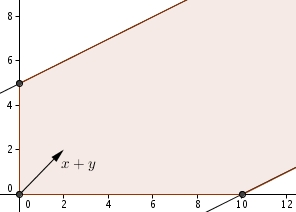
\includegraphics{ex_unbound.jpg}
\end{minipage}
This dictionary is feasible and all coefficients of $y$ are non-negative. 
This means that $y$ can increase unboundedly, 
yielding arbitrarily high values for the objective.
The command \verb|pivot|, which can pick a suitable pivot itself,
discovers this:
\begin{alltt}
pplex> pivot
Program is unbounded.
\end{alltt}

\subsection{Introduction into Sensitivity Analysis}

Once an optimum is found, it is natural to ask how sensitive it is to the accuracy of the available data. 
As an introduction into sensitivity analysis, the lecturer may for example ask the students: 
How much can we fiddle with the coefficients in the objective function without changing the optimal solution?
Students can use \texttt{pplex} to experiment with the optimal dictionary.
Consider for example the following variation of our first example,
where the objective and the first inequality are almost parallel:
\begin{alltt}
pplex> read input/nik9.lps
Read input/nik9.lps OK.

pplex> show        
 \(\zeta\) =       + 2.01x +      y
w1 =  6.00 - 2.00x -      y
w2 = 40.00 - 7.00x - 13.00y

pplex> pivot
 \(\zeta\) =  6.03 - 1.01w1 - 0.00y
 x =  3.00 - 0.50w1 - 0.50y
w2 = 19.00 + 3.50w1 - 9.50y
\end{alltt}
The optimal solution is not longer (2,2), but (3,0). 
Note the rounding error in the coefficients of $w_1$ and $y$ in the objective.
Pedagogically, an ideal occasion to introduce another feature of \url{pplex}: 
\begin{alltt}
pplex> show primal 3
 \(\zeta\) =  6.030 - 1.005w1 - 0.005y
 x =  3.000 - 0.500w1 - 0.500y
w2 = 19.000 + 3.500w1 - 9.500y
\end{alltt}
Increasing the precision eliminates the rounding error here.

\section{Work in Progress}\label{sec:future}
 
We are currently finishing a graphical interface illustrating \url{pplex} working on programs with two variables. 
The graphical illustration shows the feasible
region and highlights the vertex with the incumbent basic solution (see Figure~\ref{fig:ex_gui}).

An interesting extension is the case of \emph{unbound} variables, that is, variables that may take
negative values. The standard solution is to substitute $u = x-y$ for an unbound variable $u$,
where $x$ and $y$ are two new, non-negative variables. In the geometrical interpretation however, one would
prefer to see $u$ and stay in two dimensions.

Once this has been accomplished, we plan to implement a graphical
illustration for linear programs in three variables.

We will make an effort to keep \url{pplex} up to date and will support 
future standard formats for LP programs upon request.

\bibliographystyle{abbrv}
\begin{thebibliography}{99}
\bibitem{CiSaE2000} Computing in Science and Engineering, volume 2, no. 1, 2000.

\bibitem{Vanderbei} R.J.~Vanderbei, 
\emph{Linear Programming, Foundations and Extensions},
3rd edition, Kluwer, 2008.

\bibitem{Chvatal} V.~Chv\'atal,
\emph{Linear Programming},
W.H.~Freeman and Company, 1983.

\bibitem{pplex}
\url{https://github.com/andern/lpped/}

\bibitem{GNUGPL}
\url{http://www.gnu.org/licenses/}

\bibitem{SimplexPivotTool}
\url{http://campuscgi.princeton.edu/~rvdb/JAVA/pivot/simple.html}

\bibitem{AdvancedPivotTool}
\url{http://campuscgi.princeton.edu/~rvdb/JAVA/pivot/advanced.html}

\end{thebibliography}

\begin{figure}[htpb]
	\begin{center}
		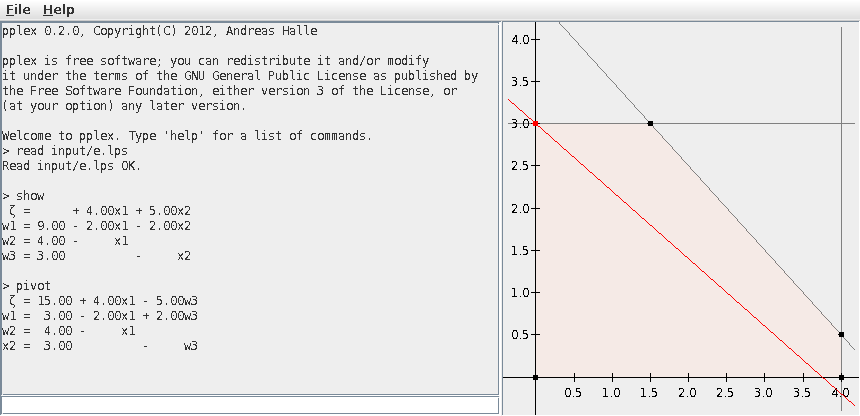
\includegraphics[width=\textwidth]{ex_gui.jpg}
	\end{center}
	\caption{Example of the Graphical User Interface}
	\label{fig:ex_gui}
\end{figure}

\end{document}
